\documentclass{article}
\usepackage[utf8]{inputenc}

% incluir imagens
\usepackage{graphicx}
\graphicspath{ {./images/} }

\title{Projeto Termômetro por um Diodo}
\author{Henrique Poleselo e Rodrigo Canário}
\date{UFBA - March 2019}

\begin{document}

\maketitle

\section{Introdução}
O objetivo deste trabalho é integrar o conhecimento visto na disciplina Dispositivos Eletrônicos sobre diodos e reguladores de tensão juntamente com Eletrônica Digital para a implementação de circuitos em FPGA.
Usando um diodo semicondutor, seguindo a sua função característica do modelo real, conseguimos relacionar temperatura com os níveis de tensão aplicado ao mesmo. Partindo deste principio conseguimos construir um termomêtro digital.

\section{Embasamento Teórico}
 O fenômeno que exploraremos é devido ao efeito Peltier, que com a aplicação de uma tensão, é criado um gradiente de temperatura que varia juntamente com a corrente. (Fenômeno termoelétrico).
\begin{center}
    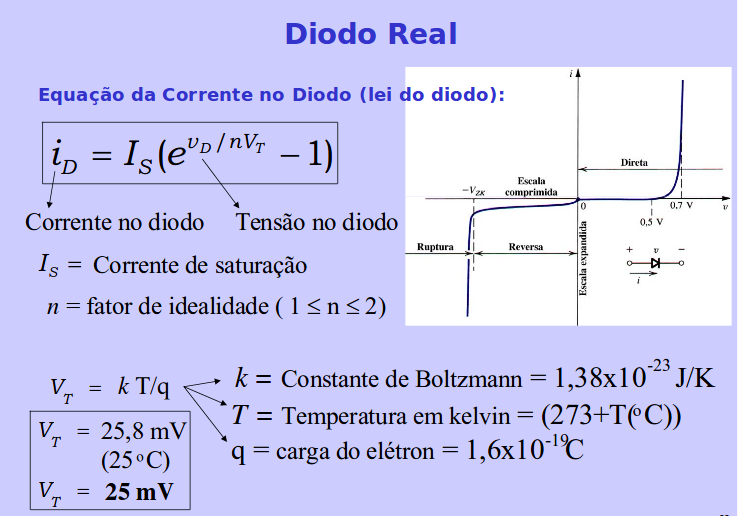
\includegraphics[scale=0.5]{images/img1.png}
    Imagem 1: Modelo do diodo real
\end{center}

\section{Estrutura do projeto}
O trabalho começa no FPGA, onde iremos implementar um algorítmo de Aproximações Sucessivas, i.e um conversor analógico digital. A saída do FPGA (pinos 3.3V) mandando sinais para uma rede R2R

\section{Simulação Conversor AD}
Usaremos as redes R-2R, que nos fornecem a possibilidade de conseguir variar níveis de tensão de acordo com as disposições dos resistores, i.e usando uma rede R-2R de 7 bits obteremos: 2(elevado)7 128 valores possiveis pra dividir a tensão de entrada. Como queremos medir de 0 100 graus com passo de 1 grau, então um R-2R de 7 bits será suficiente. Na saída da rede R2R iremos ter um ampop comparador para pegar esses valores de tensão e iremos "filtra-lo". Assim, teremos uma relação tensão-temperatura.

Queremos 12.7V na saída do ampop, começamos alimentando o AMPOP com 12.7V porém a saída, devido à perdas e à todo nosso sistema, possuia sempre aproximadamente -2V do que era inserido. Ou seja, precisávamos aumentar a entrada pra 14.7V de forma que ajustasse a saída do amplificador operacional com 12.7V. Após o encontro com Marcio vimos que de fato é um jargão: se você quer uma saída x de um amplificador operacional, alimente com x + 2V de forma a obter seu x na saída.

% inserir foto da simulacao


\section{Montagem Conversor AD}
Alimentação de tensão simétrica: precisavamos dos +14.7V e -14.7V para a alimentação do Ampop, para isso usamos a fonte de bancada que possui duas saídas de tensão, como mostrado na foto abaixo.
\begin{center}
    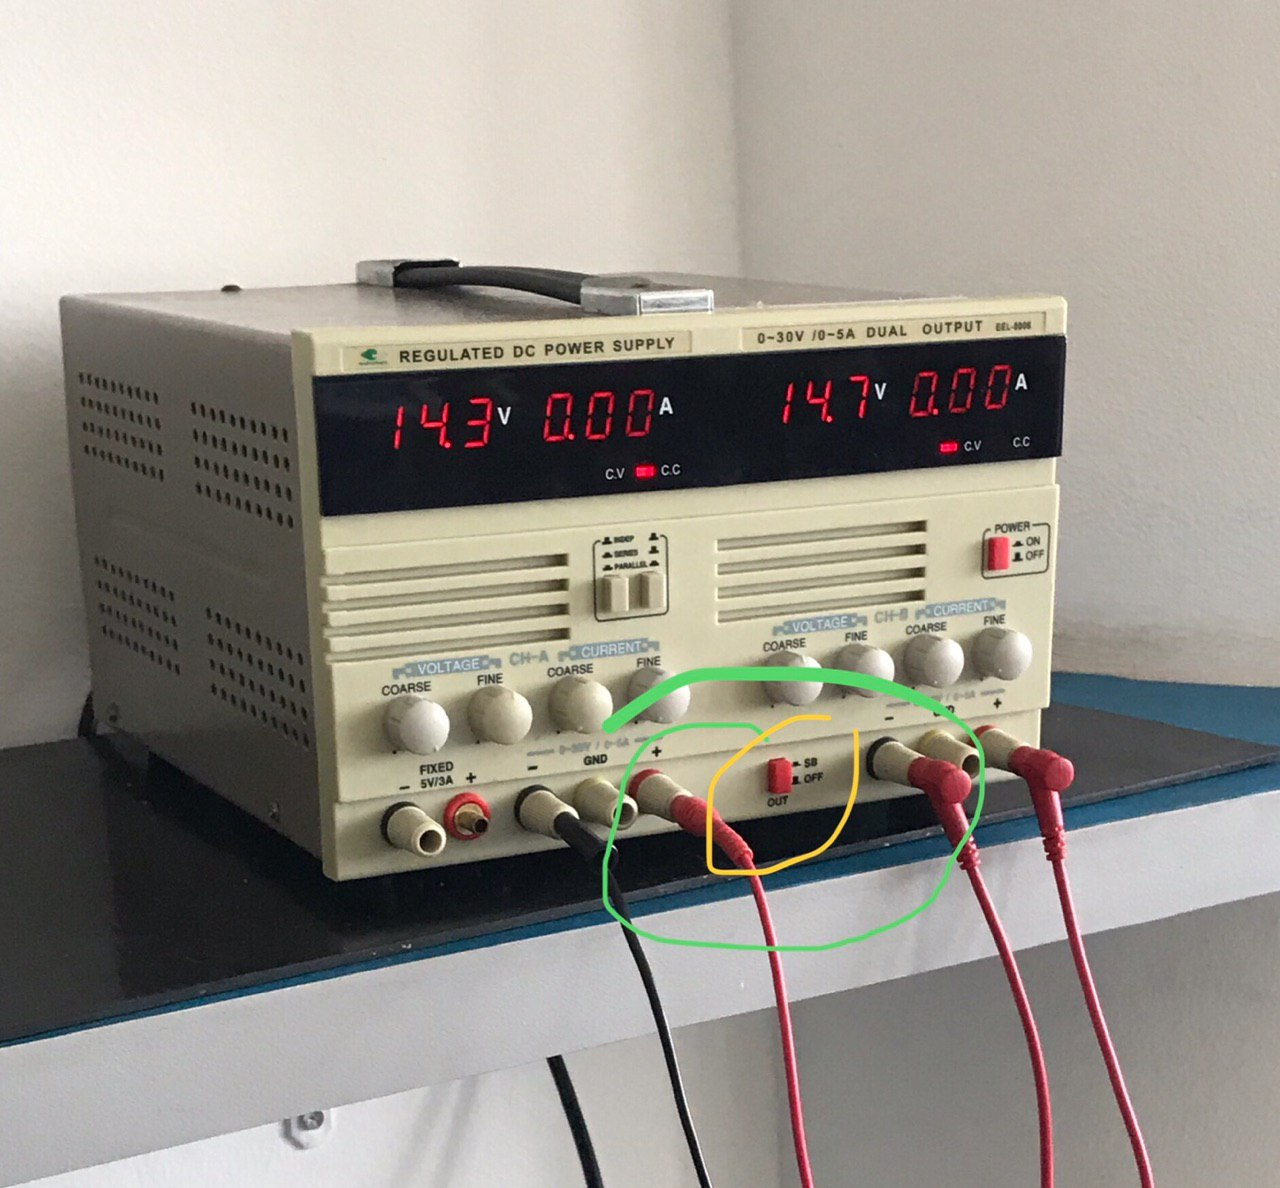
\includegraphics[scale=0.2]{images/fonte.jpeg}
    
    Imagem 2: Fonte de bancada com duas saídas.
\end{center}

Para obter a tensão simétrica precisamos realizar a ligação indicada pelo verde na foto, i.e (+ com -), essa ligação será nosso novo 0. enquanto que o cabo preto na extrema esquerda será nosso menor nível de tensão, que é -15V. Para a configuração ficar correta precisamos apertar o botão vermelho que está circulado em amarelo na imagem acima (ele ativa a ligação interna da fonte pra criar uma fonte simétrica). PS: acabmos errando isso no nosso experimento mas nessa fonte de bancada, elas funcionam sempre como uma "fonte de potência", i.e não adianta só fornecer tensão ao circuito, e sim fornecer o mínimo de corrente também (seguindo a relação $P=VI$) de forma que o circuito em questão seja realmente alimentado.

\begin{center}
    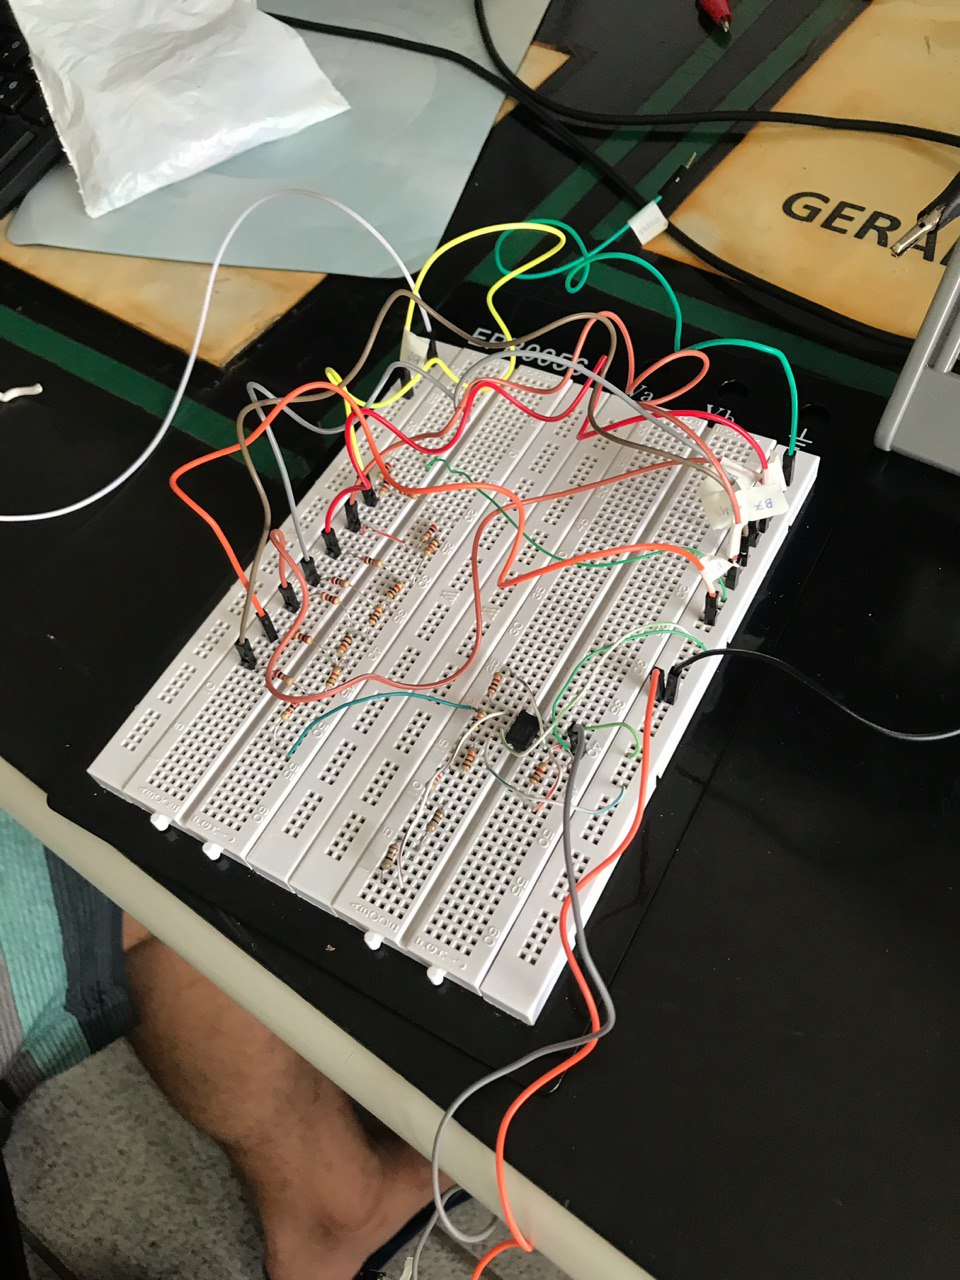
\includegraphics[scale=0.2]{images/montagem_dac.jpeg}
    
    Imagem 3: Montagem do DAC na protoboard.
\end{center}

\section{Caracterização da Curva}
Sabe-se que pra um diodo convencional, a corrente mínima necessária pra sua operação é $20mA$. Como no nosso projeto já há uma tensão alimentando todo o sistema, que é de 12.7V, usaremos a mesma pra alimentar o circuito de sensoriamento, i.e o diodo e o resistor associado para o controle da corrente $Id$. Então, pela lei de Ohm conseguimos determinar qual a resistência necessária: $R=V/I$ $R=12.7/20*10^10-3$

Iremos medir a temperatura usando um termopar, o termopar em questão é um dispositivo que é ligado diretamente ao multímetro e consegue medir a temperatura com uma certa precisão. O termopar em questão foi calibrado pra ser utilizado com o multímetro já mostrado.

\begin{center}
    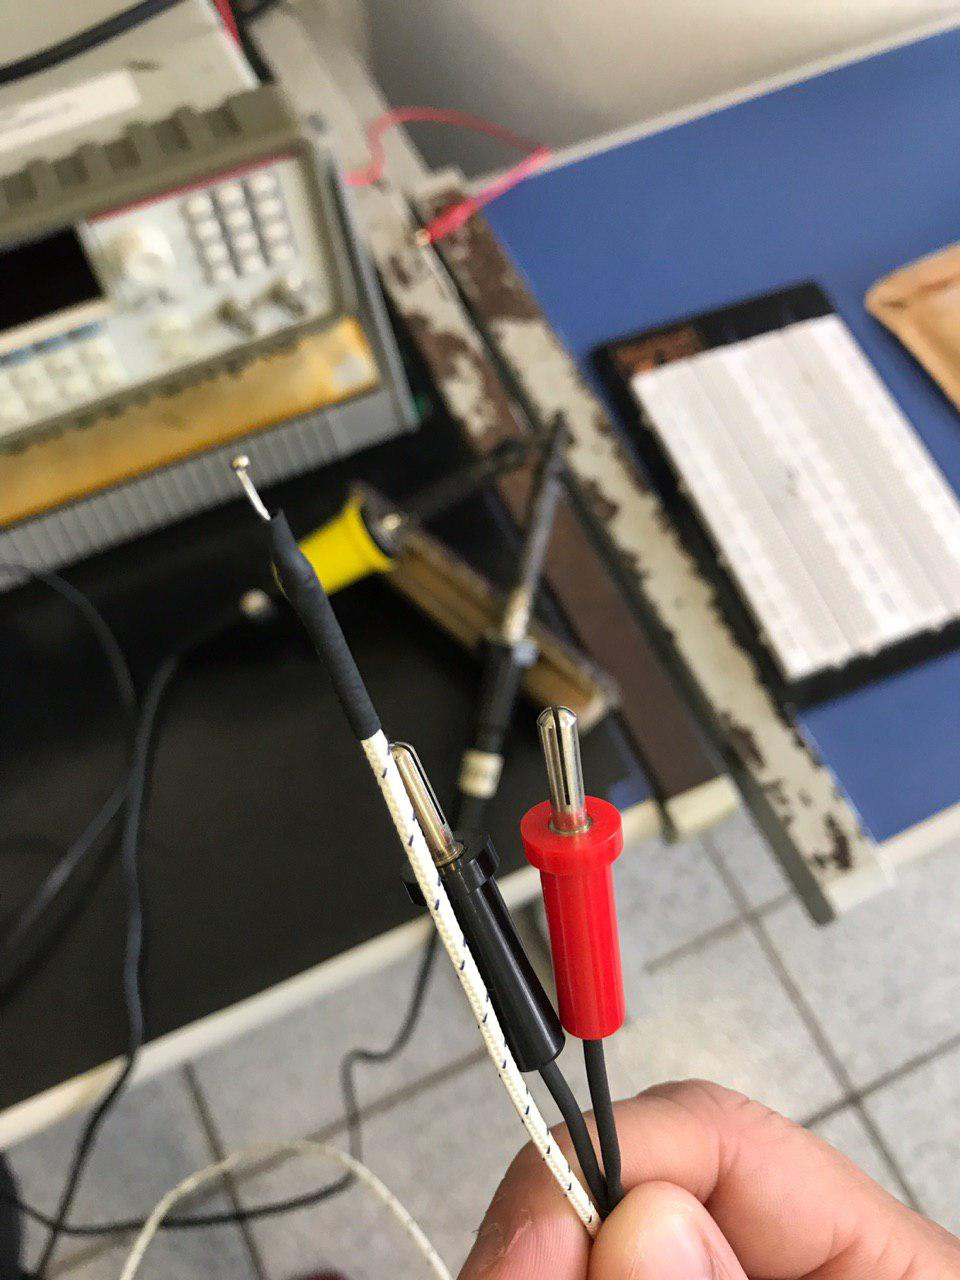
\includegraphics[scale=0.2]{images/termopar.jpg}
    
    Imagem 4: Termopar, note que a ponta em preto possui um contato, este ficará sempre em contato com o diodo para medir a temperatura no diodo.
\end{center}

Colocamos o termopar, usamos um resistor de 680 pois era o que havia disponível, soldamos as pontas do diodo com fios maiores pra facilitar a mobilidade pra medição de temperatura. Como o termopar está junto com o diodo (em toque), movimentamos o diodo e colocamos perto de um ferro de solda, o valor da temperatura aumenta enquanto que o valor da tensão no osciloscópio diminui... isso pois ambos são inversamente proporcionais.
Na prática usamos 680 ohms e 12.4v
Tabela desses valores


\end{document}
